\section{Latent World Models for Planning and Control}
\label{sec:latent_world_models}

Latent world models shift the central objective from predicting videos to learning compact dynamics that are useful for decision making. The previous sections moved from pixels to objects and relations; this section considers a different abstraction: a learned state that may not be visually interpretable, but can support planning, policy learning, or policy evolution. In this branch, images are compressed into latent variables, dynamics are learned over those variables, and control is evaluated through returns or planning success rather than only frame reconstruction. This shift is crucial for predictive world models from video because a visually accurate rollout is not always the most efficient representation for choosing actions.

\begin{figure}[t]
\centering
\begin{tikzpicture}[
  point/.style={circle, draw, fill=white, inner sep=2pt},
  label/.style={align=center, font=\small},
  note/.style={align=center, font=\scriptsize, text width=2.7cm}
]
  \draw[thick, -Latex] (0,0) -- (9,0) node[right, font=\small] {higher visual fidelity};
  \draw[thick, -Latex] (0,0) -- (0,3.6) node[above, align=center, font=\small] {higher\\abstraction};
  \draw[very thick, color=black!70] (0.8,3.0) .. controls (3.0,2.2) and (5.7,1.2) .. (8.2,0.55);
  \node[point, fill=orange!15] (latent) at (1.2,2.85) {};
  \node[label, above=3pt of latent] {Latent\\states};
  \node[note, below=8pt of latent] {efficient planning;\\may discard details};
  \node[point, fill=green!15] (object) at (4.1,1.85) {};
  \node[label, above=3pt of object] {Object-centric\\structure};
  \node[note, below=8pt of object] {interpretable relations;\\often assumes structure};
  \node[point, fill=red!12] (diff) at (7.6,0.75) {};
  \node[label, above=3pt of diff] {Pixels /\\diffusion};
  \node[note, below=8pt of diff] {rich details;\\higher cost and harder physics};
\end{tikzpicture}
\caption{The abstraction-fidelity trade-off. Latent models emphasize compact state for planning, object-centric models add interpretable structure, and pixel or diffusion models preserve visual detail but require stronger evaluation for rollout validity and physical consistency.}
\label{fig:abstraction_fidelity}
\end{figure}

\subsection{From Video Rollouts to Compact Latent Simulators}

The early recurrent world-model formulation crystallized the idea that a learned latent model can act as a simulator for downstream control. The model factorizes perception, memory, and action into a VAE, an MDN-RNN, and a controller, compressing observations into latent vectors and predicting future latent dynamics rather than rolling pixels forward directly \cite{ha2018_world_models_prov}. In this view, the world model is not merely a video predictor with a smaller output space. It is a representation of the environment that can be queried by a policy, optimized inside, or used as a surrogate environment for behavior search.

This modular formulation also exposes a recurring tension in latent world modeling. Policies can be trained inside a hallucinated environment and transferred back to the real one, but this makes simulator fidelity a central concern \cite{ha2018_world_models_prov}. If the learned dynamics are inaccurate in control-relevant regions, the controller may exploit model errors or fail when transferred. This concern is best treated as a limitation and open question rather than as a fully characterized failure mode. The section therefore treats latent simulators as powerful control substrates whose reliability must be judged by how they are used, not only by how well they reconstruct observations.

Token-based interactive world models extend this latent-simulator idea by replacing continuous recurrent states with discrete visual or interaction tokens. iVideoGPT is included in this survey as a recent bridge between VideoGPT-style tokenized video generation and interactive world modeling \cite{wu2024ivideogpt}. Its role here is to mark a design direction in which autoregressive token dynamics become part of the world-model family, not to suggest that token models supersede the recurrent VAE/RNN or RSSM lineage.

\subsection{RSSM Dynamics and Online Planning}

PlaNet made the latent-control formulation more systematic by planning directly in a recurrent state-space model. Its RSSM combines deterministic memory with stochastic latent variables, learns observation and reward models, and performs online model-predictive control by searching candidate action sequences in latent space \cite{hafner2019_planet_prov}. Figure~\ref{fig:planet-rssm} illustrates the RSSM design used for compact latent planning. This design separates the role of image generation from the role of decision making: decoded images may be useful for training or diagnostics, but planning itself uses latent states and predicted rewards. In the taxonomy of this survey, PlaNet therefore marks a clear move from image-space prediction toward compact state dynamics for action selection.

\begin{figure}[t]
    \centering
    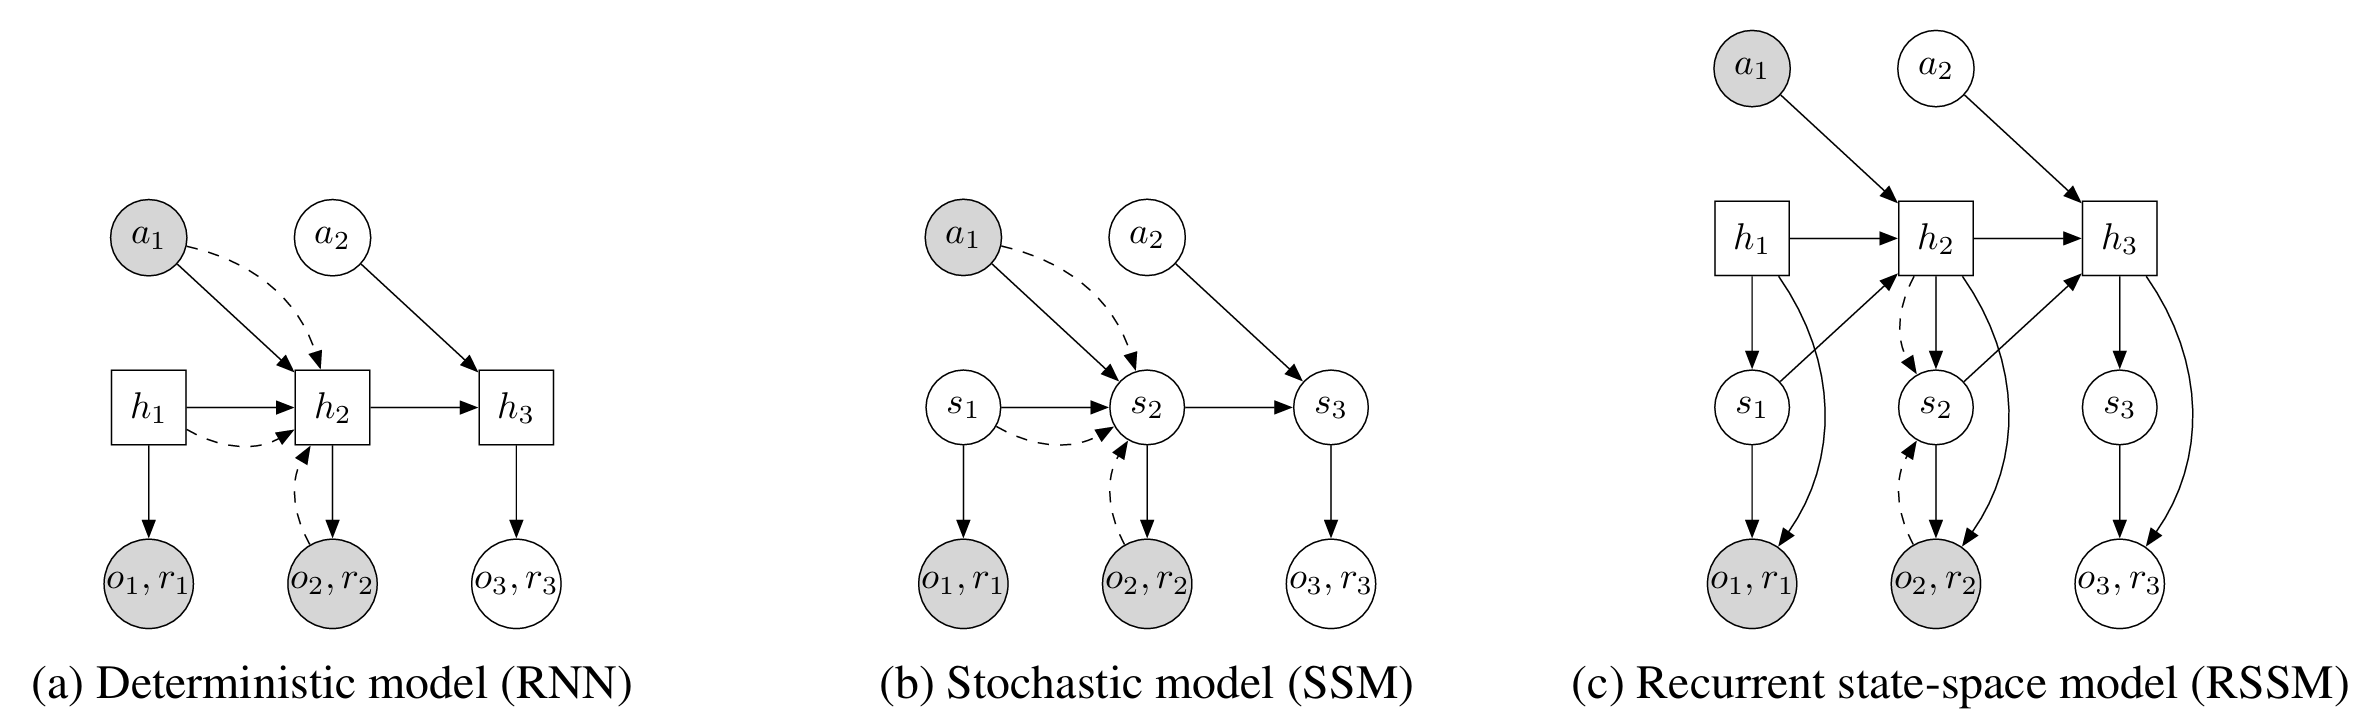
\includegraphics[width=0.88\linewidth]{../figures/planet_rssm.png}
    \caption{Recurrent state-space modeling for latent planning. PlaNet compares deterministic recurrent dynamics, stochastic state-space dynamics, and a recurrent state-space model that combines deterministic memory with stochastic latent variables. The RSSM design enables planning over compact latent states rather than over full image rollouts. Reproduced/adapted from Hafner et al.~\cite{hafner2019_planet_prov}.}
    \label{fig:planet-rssm}
\end{figure}

RSSM-style models also illustrate why the internal structure of the latent state matters. PlaNet's deterministic and stochastic components are important for performance, suggesting that latent world models need both memory for partial observability and uncertainty-aware state variables for prediction \cite{hafner2019_planet_prov}. This is not the same as the stochastic video-prediction problem in Section~\ref{sec:video_prediction}: here, uncertainty is embedded in a control-oriented state that is trained with observation and reward objectives. The relevant question becomes whether the latent state preserves the information needed for planning, not whether every generated frame is visually sharp.

Feature-space predictive models offer a different contrast to RSSM-style generative latent states. V-JEPA 2 is a self-supervised video model for understanding, prediction, and planning, with a latent representation rather than an explicit pixel decoder at the center of the discussion \cite{assran2025vjepa2_prov}. This makes it useful for comparing generative latent prediction with non-generative feature prediction. The cautious methodological claim is that feature-space predictors raise the question of whether planning-relevant state can be learned without reconstructing observations at every step.

\subsection{Latent Imagination and Policy Learning}

Dreamer changes the role of the latent model from an online planner to an imagination engine for policy learning. Instead of searching over action sequences at each decision point, Dreamer trains an actor and critic from imagined latent trajectories, using gradients through the learned dynamics and value estimates \cite{hafner2020_dreamer_prov}. This amortizes decision making into a learned policy and makes the world model a training substrate for long-horizon behavior. The conceptual shift is important: the learned dynamics are no longer only a model to plan through at test time, but a generator of imagined experience for updating behavior.

This imagination-based formulation strengthens the case that world-model evaluation differs from visual reconstruction quality. Dreamer is evaluated through visual-control performance and data efficiency, emphasizing behavior learning through latent imagination rather than pixel-space rollout fidelity \cite{hafner2020_dreamer_prov}. Together with PlaNet and the recurrent world-model formulation, this supports the survey's core latent-model claim: compact predictive states can make video-based world modeling useful for planning or policy learning \cite{ha2018_world_models_prov,hafner2019_planet_prov,hafner2020_dreamer_prov}. However, return-based evaluation still does not guarantee physical faithfulness or open-ended simulation quality. A latent model can be useful for a reward-defined task while remaining weak as a general physical simulator.

\subsection{Discrete, Token, Robotic, and Feature-Space Extensions}

Several important modern extensions belong in this conceptual family, including discrete latent world models, transformer or token-based world models, physical robot world models, feature-space planning with pretrained visual representations, and contextualized world-model pretraining from in-the-wild videos. DreamerV2, IRIS, DayDreamer, DINO-WM, ContextWM, iVideoGPT, and V-JEPA 2 are all relevant to this wider design space \cite{hafner2021_dreamerv2_prov,micheli2023_iris_prov,wu2022_daydreamer_prov,zhou2025_dino_wm_prov,wu2023_contextwm_prov,wu2024ivideogpt,assran2025vjepa2_prov}. This section uses them to clarify comparison axes for latent world models rather than to make a detailed cross-paper ranking.

The comparison axes are clear. First, discrete tokens and continuous latent states make different commitments about compression, rollout, and error accumulation. Second, generative latent prediction and non-generative feature prediction differ in whether the model must reconstruct observations or only preserve predictive state. Third, small-domain world models and large-scale video-pretrained models differ in the data regime from which their dynamics are learned. These axes make iVideoGPT and V-JEPA 2 useful additions to the survey's map, but not replacements for PlaNet and Dreamer as the foundational lineage. They should be compared carefully before being folded into stronger claims about the field as a whole.

\subsection{Limits and Transition to Image-Space World Models}

Latent world models trade visual detail for compactness and control utility. This is often a strength: planning in latent space can avoid expensive image rollouts, and actor-critic imagination can reuse a learned model to generate many behavior-learning trajectories \cite{hafner2019_planet_prov,hafner2020_dreamer_prov}. But the same abstraction creates limitations. Latent states are optimized around reconstruction, reward, value, or control objectives, so they may discard details that later matter for action. They are also typically evaluated in specific environments with defined rewards, leaving open questions about physical abstraction, compounding model error, simulator exploitation, and transfer to more complex real-world video.

The abstraction-fidelity trade-off motivates the next section on image-space and diffusion-based world models. PlaNet and Dreamer show why compact latent dynamics are attractive for planning and policy learning; DIAMOND, by contrast, argues that preserving image-space visual details can improve downstream reinforcement learning in Atari \cite{hafner2019_planet_prov,hafner2020_dreamer_prov,alonso2024_diamond_prov}. The transition is therefore not a simple progression from worse to better representations. It is a shift in design pressure: latent models emphasize efficient predictive state for control, while diffusion and interactive models revisit whether richer image-space generation or controllable video synthesis can preserve information that compact latents may lose.

The latent-model family has also diversified internally. Continuous RSSM states, discrete token models, and feature-space predictors occupy different points in the design space, and each raises different evaluation questions about planning utility, physical abstraction, and transfer. The survey therefore treats modern token and feature-space models as complementary pressure tests for the latent-world-model framework, while keeping the core evidence grounded in the recurrent world-model, PlaNet, and Dreamer lineages \cite{ha2018_world_models_prov,hafner2019_planet_prov,hafner2020_dreamer_prov,wu2024ivideogpt,assran2025vjepa2_prov}.
